

\tikzset{every picture/.style={line width=0.75pt}} %set default line width to 0.75pt        

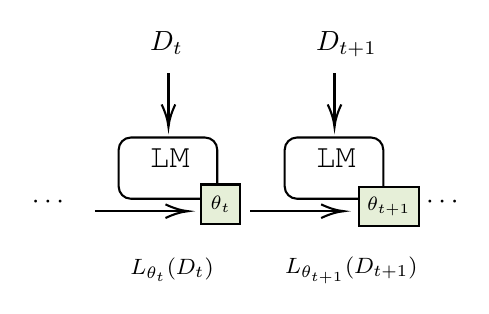
\begin{tikzpicture}[x=0.75pt,y=0.75pt,yscale=-1,xscale=1]
%uncomment if require: \path (0,300); %set diagram left start at 0, and has height of 300

%Rounded Rect [id:dp9876752621941065] 
\draw   (343,139.65) .. controls (343,136.39) and (345.64,133.75) .. (348.9,133.75) -- (384.6,133.75) .. controls (387.86,133.75) and (390.5,136.39) .. (390.5,139.65) -- (390.5,157.35) .. controls (390.5,160.61) and (387.86,163.25) .. (384.6,163.25) -- (348.9,163.25) .. controls (345.64,163.25) and (343,160.61) .. (343,157.35) -- cycle ;
%Straight Lines [id:da9054215278217996] 
\draw    (367,102.75) -- (367,126.75) ;
\draw [shift={(367,128.75)}, rotate = 270] [color={rgb, 255:red, 0; green, 0; blue, 0 }  ][line width=0.75]    (10.93,-3.29) .. controls (6.95,-1.4) and (3.31,-0.3) .. (0,0) .. controls (3.31,0.3) and (6.95,1.4) .. (10.93,3.29)   ;
%Straight Lines [id:da46451514120331305] 
\draw    (331.5,169.25) -- (374.5,169.25) ;
\draw [shift={(376.5,169.25)}, rotate = 180] [color={rgb, 255:red, 0; green, 0; blue, 0 }  ][line width=0.75]    (10.93,-3.29) .. controls (6.95,-1.4) and (3.31,-0.3) .. (0,0) .. controls (3.31,0.3) and (6.95,1.4) .. (10.93,3.29)   ;
%Rounded Rect [id:dp5047353580991751] 
\draw   (423,139.65) .. controls (423,136.39) and (425.64,133.75) .. (428.9,133.75) -- (464.6,133.75) .. controls (467.86,133.75) and (470.5,136.39) .. (470.5,139.65) -- (470.5,157.35) .. controls (470.5,160.61) and (467.86,163.25) .. (464.6,163.25) -- (428.9,163.25) .. controls (425.64,163.25) and (423,160.61) .. (423,157.35) -- cycle ;
%Straight Lines [id:da6762737459432451] 
\draw    (447,102.75) -- (447,126.75) ;
\draw [shift={(447,128.75)}, rotate = 270] [color={rgb, 255:red, 0; green, 0; blue, 0 }  ][line width=0.75]    (10.93,-3.29) .. controls (6.95,-1.4) and (3.31,-0.3) .. (0,0) .. controls (3.31,0.3) and (6.95,1.4) .. (10.93,3.29)   ;
%Straight Lines [id:da06598487354202676] 
\draw    (406.5,169.25) -- (449.5,169.25) ;
\draw [shift={(451.5,169.25)}, rotate = 180] [color={rgb, 255:red, 0; green, 0; blue, 0 }  ][line width=0.75]    (10.93,-3.29) .. controls (6.95,-1.4) and (3.31,-0.3) .. (0,0) .. controls (3.31,0.3) and (6.95,1.4) .. (10.93,3.29)   ;

% Text Node
\draw (356.67,81.33) node [anchor=north west][inner sep=0.75pt]   [align=left] {$\displaystyle D_{t}$};
% Text Node
\draw  [fill={rgb, 255:red, 230; green, 239; blue, 216 }  ,fill opacity=1 ]  (382.61,156.39) -- (401.61,156.39) -- (401.61,175.39) -- (382.61,175.39) -- cycle  ;
\draw (392.11,165.89) node  [font=\scriptsize] [align=left] {$\displaystyle \theta _{t}$};
% Text Node
\draw (356.47,137.67) node [anchor=north west][inner sep=0.75pt]  [font=\large] [align=left] {{\fontfamily{pcr}\selectfont LM}};
% Text Node
\draw (436.67,81.33) node [anchor=north west][inner sep=0.75pt]   [align=left] {$\displaystyle D_{t+1}$};
% Text Node
\draw  [fill={rgb, 255:red, 230; green, 239; blue, 216 }  ,fill opacity=1 ]  (458.61,157.39) -- (487.61,157.39) -- (487.61,176.39) -- (458.61,176.39) -- cycle  ;
\draw (473.11,166.89) node  [font=\scriptsize] [align=left] {$\displaystyle \theta _{t+1}$};
% Text Node
\draw (347.17,190.33) node [anchor=north west][inner sep=0.75pt]  [font=\footnotesize] [align=left] {$\displaystyle L_{\theta _{t}}( D_{t})$};
% Text Node
\draw (421.67,189.83) node [anchor=north west][inner sep=0.75pt]  [font=\footnotesize] [align=left] {$\displaystyle L_{\theta _{t+1}}( D_{t+1})$};
% Text Node
\draw (299.67,160.33) node [anchor=north west][inner sep=0.75pt]   [align=left] {$\displaystyle \cdots $};
% Text Node
\draw (489.67,160.33) node [anchor=north west][inner sep=0.75pt]   [align=left] {$\displaystyle \cdots $};
% Text Node
\draw (436.47,137.67) node [anchor=north west][inner sep=0.75pt]  [font=\large] [align=left] {{\fontfamily{pcr}\selectfont LM}};


\end{tikzpicture}
